\chapter{Integrated Circuitry Design}
This chapter presents the design of the read-out circuit and the post-simulation results.


\section{Fronted Circuit Design}
The review of the source follower in section.\ref{section:SF} suggests the constant current method for the circuit of DC-Sweep mode.
The data analysis from chapter 3 supports it by the linear relation between $I_D$ and $g_m$.
However, section.\ref{sec:AC} shows that source follower is not suitable for transient measurement.
It alternatively recommends the circuit in Fig.\ref{fig:lockin} which measures the transient current signal and converts it into a voltage output.

The fronted circuit combined these two methods into one circuit structure with two modes available: the DC-Sweep mode and the Transient Measurement mode.

\subsection{The DC-Sweep mode}
\begin{figure}[!htbp]
    \centering
    \includegraphics[width=0.4\textwidth] {images/chapter5/DCMode.png}
    \caption{The fronted circuit operated in DC-Sweep mode.}
    \label{fig:DCmode}
\end{figure}
Fig.\ref{fig:DCmode} is the fronted circuit operated in the DC-Sweep mode.
The switch turns the circuit into the DC-Sweep mode by connecting the output of OP with the gate of nanowire.

As in the source follower, our circuit contains a biasing current source (Ibias) for controlling the $I_D$.
The difference is that the Ibias inputs the current into drain instead of source.
In addition, we employs the transimpedance amplifier (TIA) from section.\ref{sec:AC} (\cite{Jlockin}).
Its output is connected to a rail-to-rail OP amplifier to form a negative feedback loop.
When $I_D$ is less than Ibias, the output voltage of TIA falls and the gate voltage $V_G$ rises to increase $I_D$.
On the contrary, output voltage of TIA rises and the gate voltage ($V_G$) drops if Ibias is smaller than $I_D$.
Finally, the feedback mechanism forces $I_D$ to be the same as Ibias by adjusting $V_G$ automatically.


\subsection{Transient Measurement mode} \label{sec:TrM}

\begin{figure}[!htbp]
    \centering
    \begin{minipage}[t]{0.4\textwidth}
        \includegraphics[width=1\textwidth] {images/chapter5/ACMode.png}
        \raggedleft
        (a)
    \end{minipage}
    \hfill
    \begin{minipage}[t]{0.4\textwidth}
        \includegraphics[width=1\textwidth] {images/chapter5/ACMode_sine.png}
        \raggedleft
        (b)
    \end{minipage}
    \caption{Two usage ((a), (b)) of the fronted circuit operatd in transient measurement mode.}
    \label{fig:ACmode}
\end{figure}

In Fig.\ref{fig:ACmode}(a), the switch turns to a simple voltage source (Vg) that provides a constant gate voltage.
The feedback OP is nonfunctional in this mode.
When performing measurement, we directly find how the output voltage ($V_{out}$) changes with the biomolecule concentration.
This output voltage will be sent into a second stage circuit for further amplification.

\paragraph*{Another Usage of Transient Measurement mode}
There is another method to perform measurement with the Transient Measurement mode, which resembles the measurement in \cite{Jlockin}.
This method measures the $g_m$ of the nanowire.
As shown in Fig.\ref{fig:ACmode}(b), a sinusoidal signal with an amplitude of $v_s$ is sent to the source of the nanowire.
The output response ($V_{out}$) is a sinusoidal signal at the same frequency with an amplitude equaling to $v_sg_m \times R_{TIA}$.
The values of Ibias and Vg can be arbitrary.
But one need to be aware that their values should not cause the output of TIA or the second-stage circuit to saturate.

\subsection{Dealing with the Disparity Problem}
As mentioned in chapter 1, we combine the DC-Sweep mode and Transient Measurement mode to perform a disparity-resisting measurement.

\paragraph*{Method Procedure}
Assuming there are two nanowire devices and the disparity problem exists between them.
Initially, we use these element to perform the $I_D$-$V_G$ sweep in the DC-Sweep mode.
We use the DC-Sweep results to find the $g_m$ of each device. ($g_m = \frac{\partial I_D}{\partial V_G}$)
When we turns to the Transient Measurement mode, we bias these two devices under the same $g_m$ by setting Ibias and Vg correspondingly.
After the buffer solutions, the same voltage difference at the output ($V_{out}$) should be detected because the two devices have the same $g_m$.
Before a new solution is added, we return to the DC-Sweep mode again.
This is for finding the new biasing $V_G$ to reset their $I_D$ to be the same as Ibias.
This implies that every time when we enter the Transient Measurement mode, the devices always have the same $I_D$ and $g_m$ as those in the beginning of experiments.


\subsection{Design Description}
In this section, we first talk about the TIA block and focus on how we improve the detecting limits of this block.
It is followed by the design of the TIA circuit.
Then we analyze the feedback mechanism of the DC-Sweep mode and the input impedance of the circuit.
After that, we discuss the stability issue.
Finally, we show the design of the feedback OP block.

\subsubsection{Strategies for lowering current detecting limits} \label{sec:Ibias}
The TIA subcircuit in section.\ref{sec:ch2CC} is shown as Fig.\ref{fig:TIA_old}(a), we mentioned that the detecting range of $R_{NW}$ is limited by $I_{NW}$ provided by the TIA.
We now discuss the causes of the upper and lower limits, and show the strategies we use to improve them.

\begin{figure}[!htbp]
    \centering
    \begin{minipage}[t]{0.4\textwidth}
        \includegraphics[width=1.1\textwidth] {images/chapter5/TIA_olda.png}
        (a)
    \end{minipage}
    \hfill
    \begin{minipage}[t]{0.4\textwidth}
        \includegraphics[width=1\textwidth] {images/chapter5/TIA_old.png}
        (b)
    \end{minipage}
    \caption{\textbf{(a)} The transimpedance block (TIA) of the read-out circuit from \cite{Jlockin}. The circuit input a voltage signal into resistive nanowire element $R_{NW}$.
            To compare it with our circuit (Fig.\ref{fig:TIA}), we transform the voltage input into an equivalent current input in \textbf{(b)}. The $I_{NW} = (V_{Ref} - V_{in})/R_{NW}$ and $\Delta i = \Delta vi /R_{NW}$}
    \label{fig:TIA_old}
\end{figure}

\paragraph*{Lower Limit:}
In Fig.\ref{fig:TIA_old}(b), the TIA output voltage is:
\begin{equation}
    V_{TIA} = V_{Ref} + I_{NW}R_{TIA} + \Delta iR_{TIA}
    \label{eq:TIA_old}
\end{equation}
Two reasons relate to a large offset current $I_{NW}$.
One is that the output current provided by the TIA is restricted by design.
The other is that the restriction of the current flowing through the resistor $R_{TIA}$:
\begin{align}
    \frac{V_{Ref} - VSS}{R_{TIA}} < I_{NW} < \frac{VDD - V_{Ref}}{R_{TIA}}
\end{align}
Both reasons lead to the output saturation of TIA.

A naive way to handle the first one is to increase the maximum output current the TIA can provide.
The disadvantage of this method is the increase in power consumption and chip area.
As for the second one, using smaller $R_{TIA}$ can release the restriction on $I_{NW}$.
Unfortunately, this is unpreferable because it reduces the current-to-voltage gain of the TIA.

Our strategy for decreasing the lower limit is to utilize the biasing current source (Ibias) of nanowire.
As shown in Fig.\ref{fig:TIA}, Eq.(\ref{eq:TIA_old}) is transformed into:
\begin{equation}
    V_{TIA} = V_{Ref} + (I_{NW} - I_{bias}) R_{TIA} + \Delta iR_{TIA}
    \label{eq:TIA}
\end{equation}
Now we can diminish the large $I_{NW}$ by Ibias.

In conclusion, the large offset current causes the saturation of the output of TIA.
We use the biasing current source to diminish that offset current, so as to increase the detection range.

\begin{figure}[!htbp]
    \centering
        \includegraphics[width=0.4\textwidth] {images/chapter5/TIA.png}
    \caption{}
    \label{fig:TIA}
\end{figure}
\paragraph*{Upper Limit:}
The upper limit depends on the output resolution.
When the input current signal $\Delta i$ in Fig.\ref{fig:TIA} is too small, the output response may be defeated by the noise.
This may be solved by increasing the SNR through a larger $R_{TIA}$.
However, the chip area constrains the size of resistors.
In our circuit design, it is hard to make a wide linear range resistor with resistance value out of $100k\Omega$.
Furthermore, even if the resistor can be greater, one need to concern for the noise brought by the large resistance.

Our strategy is to boost the SNR of TIA by designing its input MOSFETs with a large area.
We also amplify the output signal through the second-stage circuit.

\subsubsection{TIA (Transimpedance Amplifier) Design}

\begin{figure}[!htbp]
    \centering
    \begin{minipage}[t]{0.4\textwidth}
        \includegraphics[width=1\textwidth] {images/chapter5/TIA_block.png}
        \raggedleft
        (a)
    \end{minipage}
    \hfill
    \begin{minipage}[t]{0.5\textwidth}
        \includegraphics[width=1\textwidth] {images/chapter5/TIA_sch.png}
        \raggedleft
        (b)
    \end{minipage}
    \caption{(a)The transimpedance block and the (b) schematic}
    \label{fig:TIA_sch}
\end{figure}
Fig.\ref{fig:TIA_sch} shows the Transimpedance Amplifier circuit.
We implement the operational amplifier in TIA with the two-stage, differential-pair structure.
This simple structure has merits such as large output current and wide output voltage range.

Fig.\ref{fig:TIA_postSim_dc} and Fig.\ref{fig:TIA_postSim_ac} show the dc and ac post-simulation of the TIA.
Table.\ref{tb:TIAsim} summarises the simulation result.
{\color{red}not done yet!!!}
\begin{table}[!htb]
    {\fontfamily{}\fontsize{10}{14}\selectfont
    \centering
    \begin{tabular}{l|c}
        Input Current range & from $6\mu A$ to $-10\mu A$\\
        \hline
        Bandwidth & 7M Hz \\
        \hline
        Output referred noise (@10Hz) & $0.01mV$ \\
    \end{tabular}
    \caption{Post-simulation result of TIA}
    \label{tb:TIAsim}
    }
\end{table}
\begin{figure}[!htbp]
    \centering
        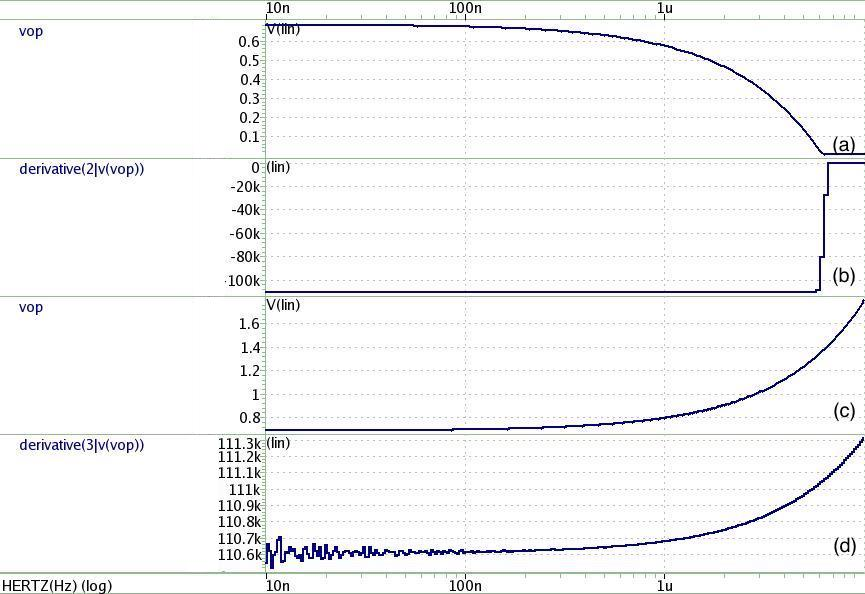
\includegraphics[width=1\textwidth] {images/chapter5/postSim/TIA_dc.png}
    \caption{The dc simulation results of TIA. The x-axis represents positive/negative input current (log scale). \textbf{(a)} is the $V_{out}$ responding to the positive input current while \textbf{(c)} is to the negative input current.
                    \textbf{(b)} and \textbf{(d)} are the derivative of $V_{out}$ of input current ($\frac{\partial V_{out}}{\partial {I_{in}}}$) from \textbf{(a)} and \textbf{(c)} respectively.}
    \label{fig:TIA_postSim_dc}
\end{figure}
\begin{figure}[!htbp]
    \centering
        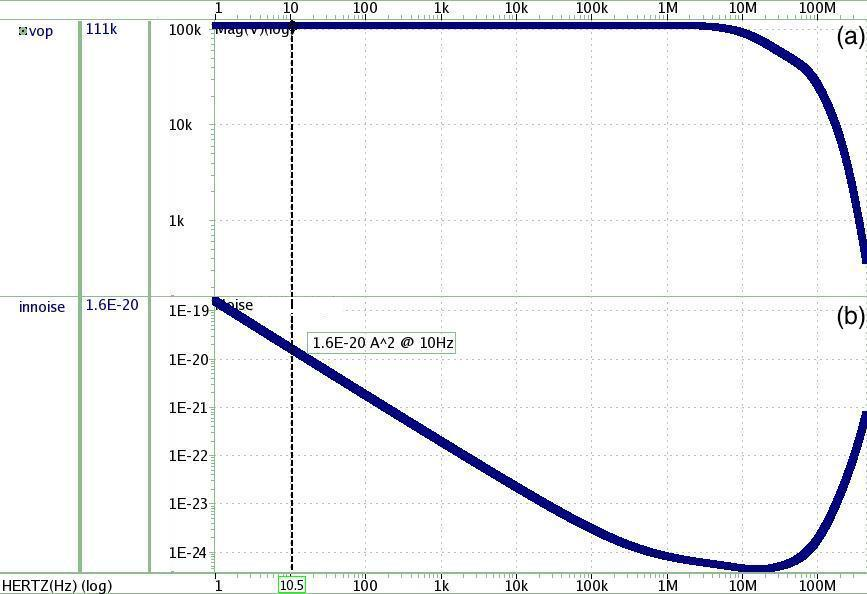
\includegraphics[width=1\textwidth] {images/chapter5/postSim/TIA_ac.png}
    \caption{The ac simulation results of TIA. The x-axis is the input signal frequency. \textbf{(a)} is the $V_{out}$ and \textbf{(b)} is the output-referred noise.}
    \label{fig:TIA_postSim_ac}
\end{figure}

\subsubsection{Feedback Mechanism} \label{sec:feedM}
The DC-Sweep mode circuit forms a negative feedback loop.
Fig.\ref{fig:feedblock} is the block diagram of the circuit.
\begin{figure}[!htbp]
    \centering
        \includegraphics[width=0.7\textwidth] {../images/chapter5/feedbackBlock.png}
    \caption{Block diagram of the DC-Sweep mode. The $Iin$ refers to the Ibias and $Vout$ refers to the output voltage of OP, which is also the gate voltage of nanowire (Fig.\ref{fig:DCmode}). The $gm(I_D)$ is the transconductance of nanowire whose values depends on $I_D$.}
    \label{fig:feedblock}
\end{figure}

From the block diagram, we can compute the loop gain ($LG$) and the transfer function ($TF$):
\begin{align}
    R_A &= R_{TIA} \times A_{OP} \\
    LG &=  R_A \times g_m \\
    TF &= \frac{V_{out}}{I_{in}} =  \frac{R_A}{1 + LG} \label{eq:TF}\\
    &\approx \frac{1}{gm} \quad \text{If LG $\geq$ 100}
\end{align}
The transfer function suggests that if we want to obtain an $I_D$-$V_G$ sweeping curve with an error less than \%1, our loop gain should be greater than 100.
According to chapter 3, the spec for $g_m$ detection ranges from $200n$ to $20u$.
This implies that $A_{OP}$ should be at least greater than 5k.
We will show in the next section that the $A_{OP}$ in the post-simulation is 10k.

{\color{red}Fig.\ref{fig:sim:TF} is the post-simulation result of the circuit.
A simple mosfet substituted for nanowire device during the simulation.
The $g_m$ of the mosfet is kept at values of $20\mu$, $2.02\mu$ and $226n$ to model the $g_m$ range of nanowire.}
We performed AC analysis by sending a small current signal to $I_{in}$ and detected the AC response of $V_{out}$.
Afterwards, we compared the $g_m$ values with the $\frac{I_{in}}{V_{out}}$.
The comparison are summarized in Table.\ref{tb:sim:TF}.



\begin{figure}[!htb]
    \centering
        \includegraphics[width=1\textwidth] {images/chapter5/postSim/feedbackMechanism.PNG}
    \caption{The simulation results of $\frac{V_{out}}{I_{in}}$}
    \label{fig:sim:TF}
\end{figure}

\begin{table}[!htb]
    {\fontfamily{}\fontsize{10}{14}\selectfont
    \centering
    \begin{tabular}{l|c|c|c}
        & $V_{out}$ & $\frac{I_{in}}{V_{out}}$ & error \\
        \hline
        $g_m$ = $20\mu$ & $50k$ & $20u$ & Unable to detect \\
        \hline
        $g_m$ = $2.02\mu$ & $495k$ & $2.02\mu$ & Unable to detect \\
        \hline
        $g_m$ = $226n$ & $4.32M$ & $231.5n$ & 1.02\%\\
    \end{tabular}
    \caption{The the comparison of $g_m$ and $\frac{I_{in}}{V_{out}}$}
    \label{tb:sim:TF}
    }
\end{table}

\subsubsection{Input Impedance (DC-Sweep mode)}
In chapter 4, we have discussed the impedance matching between the current source and the nanowire device.
Here we compute the input impedance of the circuit.

\begin{figure}[!htbp]
    \centering
        \includegraphics[width=0.4\textwidth] {images/chapter5/input_imp.png}
    \caption{}
    \label{fig:input_imp}
\end{figure}
In Fig.\ref{fig:input_imp}, we apply an input voltage $\Delta v_x$ and find the $\Delta i_x$.
The input impedance of the circuit is $\Delta v_x / \Delta i_x$.
\begin{align}
      \Delta i_x &= \quad i_D + i_{TIA} \\
      i_D &= \quad \frac{\Delta v_x}{r_{ds}} + \Delta v_xA_{TIA}A_{OP}g_m\\
      i_{TIA} &= \quad \frac {\Delta v_x}{R_{TIA} / (1 + A_{TIA})} \\
      \Delta v_x / \Delta i_x  &= \quad (\cancel{\frac{1}{r_{ds}}} + A_{TIA}A_{OP}g_m + \frac{1 + A_{TIA}}{R_{TIA}})^{-1} \\
       &= \frac{R_{TIA}}{(1 + A_{TIA})(1 + R_{TIA}{A_{OP}g_m})}  \label{eq:input_imp}
\end{align}
The $A_{TIA}$ is the gain of the opAmp in TIA block.
The $A_{OP}$ is the gain of the feedback OP.
The $r_ds$ is the drain-to-source resistance of nanowire, which is larger than $100k\Omega$.

The Eq.(\ref{eq:input_imp}) can be rewritten into:
\begin{equation}
    \frac{Z_{in}}{1 + LG}
\end{equation}
where the $Z_{in}$ is the input impedance of TIA.

The OpAmp of TIA holds the gain of 1000 (60dB), which makes the $Z_{in}$ of 100.
The LG is greater than 5k from the last section.
In our design, the Ibias is a simple pmos.
Its output impedance ranges from $1M\Omega$ to $1G\Omega$.
It is obvious that the input impedance is much smaller than the $r_{ds}$.
The result tells that the impedance matching is fine.

\subsubsection{Stability and Feedback OP Design} \label{sec:stabilityandOP}
To decide the structure of the feedback OP, we must discuss the stability of the feedback loop in the DC-Sweep mode.
The OP plays a crucial role in the stability issue because it not only decides the loop gain but also contains the dominant pole at its output.

\begin{figure}[!htbp]
    \centering
        \includegraphics[width=0.4\textwidth] {../images/chapter5/LoopGain.png}
    \caption{}
    \label{fig:loopgain}
\end{figure}

In Fig.\ref{fig:loopgain}, we mark the dominant pole ($w_{p1}$), second order dominant pole $w_{p2}$) and the zero ($w_z$).
We can write the loop gain as:
\begin{align}
    & \frac{v_f}{v_e} =  R_{TIA} \times A_{OP} \times g_m \frac{1 - s/w_z}{(1 + s/w_{p1})(1 + s/w_{p2})} \\
    & w_z = \frac{g_m}{C_{gd}}
\end{align}
The parasitic capacitance $C_{gd}$, at the conservative estimate, has a maximum value of $1pF$ (The estimation is based on the fabrication information from \cite{DN17} and \cite{C6}).
And because the lower bound of $g_m$ in our design spec (Table.\ref{tb:DCspec}) is $200n$, the $w_z$ can be as small as 20k.
To force the total loop gain to drop to 1 before $s > 2k$, we have to move the first dominant pole left.

We choose the $w_{p1}$ as the first dominant pole.
From section.\ref{sec:feedM}, we learned that the $A_{OP}$ should be larger than $5k$.
Thus, we choose a folded cascode structure which provides high output impedance and gain.

\begin{figure}[!htbp]
    \centering
    \begin{minipage}[t]{0.35\textwidth}
        \includegraphics[width=1\textwidth] {images/chapter5/OP_block.png}
        \raggedleft
        (a)
    \end{minipage}
    \hfill
    \begin{minipage}[t]{0.6\textwidth}
        \includegraphics[width=1\textwidth] {images/chapter5/OP_sch.png}
        \raggedleft
        (b)
    \end{minipage}
    \caption{(a)The feedback OP block and its (b) schematic}
    \label{fig:OP_sch}
\end{figure}

We designed a folded cascode OP with gain of 10k (80dB) and bandwidth less than 3Hz (Fig.\ref{fig:OP_sch}, Table.\ref{tb:OPsim}).
A higher gain prevents the circuit from the fabrication flaw (30\% deviation of the impedance of the $R_TIA$ in TIA block).
The low bandwidth is owing to the large capacitance (Cf) appended to the output.
This capacitance results in a lower slew rate, which is fine because the circuit is for DC signal and there is no need for high speed operation.

\begin{table}[!htb]
    {\fontfamily{}\fontsize{10}{14}\selectfont
    \centering
    \begin{tabular}{l|c}
        BandWidth & 2 Hz\\
        \hline
        Max Gain & 81dB \\
        \hline
        Output Dynamic Range & $0.45V$ - $2.6V$ \\
    \end{tabular}
    \caption{Post-simulation result of feedback OP}
    \label{tb:OPsim}
    }
\end{table}

\subsection{The Post-simulation Result of the DC-Sweep mode circuit}

\subsubsection{DC Current (Ibias) Sweep}
We swept the Current of Ibias and measured the output voltage of the feedback OP which is also the $V_G$.
We also measured the $I_D$ of the transistor.
(Because we don't have nanowire model, we performed the simulation by using an alternative mosfet.)
The curve of $I_{bias}$-$V_G$ is compared with the curve of $I_D$-$V_G$ (Fig.\ref{fig:sim:DCIcompare} (a)).
Moreover, we compare the measured $g_m$ ($\frac{I_{bias}}{V_G}$) with the intrinsic $g_m$ ($\frac{I_D}{V_G}$) (Fig.\ref{fig:sim:DCIcompare}(b)).
This is according to the section of the feedback mechanism (section.\ref{sec:feedM}).
The result in Fig.\ref{fig:sim:DCIcompare}(c) shows that the error is over 1\% when the $g_m$ of the transistor is less than $130n$.

\begin{figure}[!htbp]
    \centering
        \includegraphics[width=1\textwidth] {images/chapter5/postSim/DCIcompare_all.PNG}
    \caption{}
    \label{fig:sim:DCIcompare}
\end{figure}

\subsubsection{Bode Plot of Loop Gain and Phase}
The simulation here is according to the stability section (section.\ref{sec:stabilityandOP}).
We present the Bode plot of the loop gain and the phase (Fig.\ref{fig:sim:loopsim}).
The summarization table is also given (Table.\ref{tb:1staACsim}).
We adjusted the transistor to the specific $g_m$ values by selecting the Ibias and corresponding $V_G$.
We also appended a $1pF$ capacitance to model the $C_{gd}$.


\begin{figure}[!htbp]
    \centering
        \includegraphics[width=1\textwidth] {images/chapter5/postSim/stability_1p_fs.PNG}
    \caption{Results of the ac simulation of the loop gain and phase (Bode plot) with different $g_m$ value ($200n$, $2u$, $20u$). These $g_m$ value is selected according to the DC-Sweep mode spec we set in chapter 3 (section.\ref{sec:spec3}).}
    \label{fig:sim:loopsim}
\end{figure}


\begin{table}[!bhtp]
    {\fontfamily{}\fontsize{10}{14}\selectfont
    \centering
    \begin{tabular}{l|c|c|c}
        $g_m$ & $20\mu$ & $2\mu$ & $200n$\\
        \hline
        Loop Gain & 20k & 2k & 200\\
        \hline
        Phase Margin & 80(deg) & 78(deg) & 81 (deg) \\
    \end{tabular}
    \caption{The phase margin and loop gain of the fronted circuit}
    \label{tb:1staACsim}
    }
\end{table}

Table.\ref{tb:DCcompare} is for comparing the design spec and the simulation result.
To be noted that the upper limit of $I_D$ and $g_m$ of our circuit is unclear because they depends on two factors.
One is the gate voltage.
Tbale.\ref{tb:OPsim} shows that the maximal gate voltage that the Feedback OP can provides is $2.6V$.
The other is the current bias.
The Ibias is a simple pmos whose current is decided by an external resistor (Fig.\ref{fig:mirror}).
This current mirror structure has a maximum output current of $70\mu A$.


\begin{figure}[!htbp]
    \centering
        \includegraphics[width=0.3\textwidth] {images/chapter5/mirror.PNG}
    \caption{The current mirror structure of the current source Ibias.}
    \label{fig:mirror}
\end{figure}


\begin{table}[!htbp]
    {\fontfamily{}\fontsize{10}{14}\selectfont
    \centering
    \begin{tabular}{l|c|c}
        & Design Spec & Simulation result \\
        \hline
        $I_D$ & $100n A$ - $30\mu A$ & $> 20n A$ \\
        \hline
        $g_m$ & $200n$ - $20\mu$ & $> 130n$ \\
    \end{tabular}
    \caption{The comparison between the design spec and simulation result of the DC-Sweep mode circuit.}
    \label{tb:DCcompare}
    }
\end{table}


\FloatBarrier


\section{Second Stage Circuit Design}

We discuss the second stage circuit in this section.
To be noted that the second stage circuit is only for Transient Measurement mode.

\begin{figure}[!htbp]
    \centering
        \includegraphics[width=1\textwidth] {images/chapter5/Second.png}
    \caption{}
    \label{fig:secondStage}
\end{figure}
Fig.\ref{fig:secondStage} is the block diagram of the second stage circuit.
The analog subtractor shifts the voltage of the $V_{in}$ from $V_{Ref}$ to $V_z$.
It follows by a resistor-based non-inverting amplifier composed of a two-stage differential operational amplifier, two switches and three resistors.
The switches select the amplification rate among 100, 10 and 1.

\subsection{Analog Subtractor}

\begin{figure}[!htbp]
    \centering
        \includegraphics[width=0.5\textwidth] {../images/chapter5/Subtractor.png}
    \caption{Block diagram of the second stage circuit.}
    \label{fig:subtractor}
\end{figure}

Fig.\ref{fig:subtractor} is the schematic of our analog subtractor which references \cite{Tsubtractor}.
The output voltage equals to:
\begin{equation}
    v_x - V_{Ref} + v_z
\end{equation}

A voltage signal $\Delta v$ sent to vx induces a current difference ($\Delta i_d$) of Mx.
This current is mirrored to the diode-connected Mz by the cascode current mirror formed by M1 to M4.
The changing of the current changes the gate voltage of Mz.
And this voltage is buffered to the output by the source follower M5.

\begin{align}
    & \Delta v_{out} = \Delta v_{x}\frac{g_{mx}}{g_{mz}} - V_{Ref}\frac{g_my}{g_m5} + v_z\\
    & \Delta v_{out} = \Delta v_{x} - V_{Ref} \quad \text{For $g_{mx} = g_{mz}$; $g_{my} = g_{m5}$}
\end{align}

One of the reasons that we apply this block is because the $V_{Ref}$ is an internal voltage reference which may drift by the process variance.
We prefer the output offset voltage of the circuit to be constant and controllable.
In such a way, we shift it to $v_z$ which is controlled by an external voltage source.
Another reason is to increase the input dynamic range of the next amplifier block.
This reason will be much clearer when we start discussing the amplifier block in the next section.

We performed DC sweep on input ($v_X$) and $v_z$ at five corners to show the linear region of the circuit (Fig.\ref{fig:sim:subtractor}, Table.\ref{tb:Subtractor}).
The circuit has input dynamic range of $0.77V$ while the dynamic range for $v_z$ is $0.38V$.

To be more specific, the input dynamic range is from $-0.5V$ to $+0.2$.
When the current flowing through the TIA block is greater than $+5\mu A$ or smaller than $-2\mu A$, the output of the second stage circuit is saturated.


\begin{figure}[!htbp]
    \centering
    \begin{minipage}[t]{1\textwidth}
        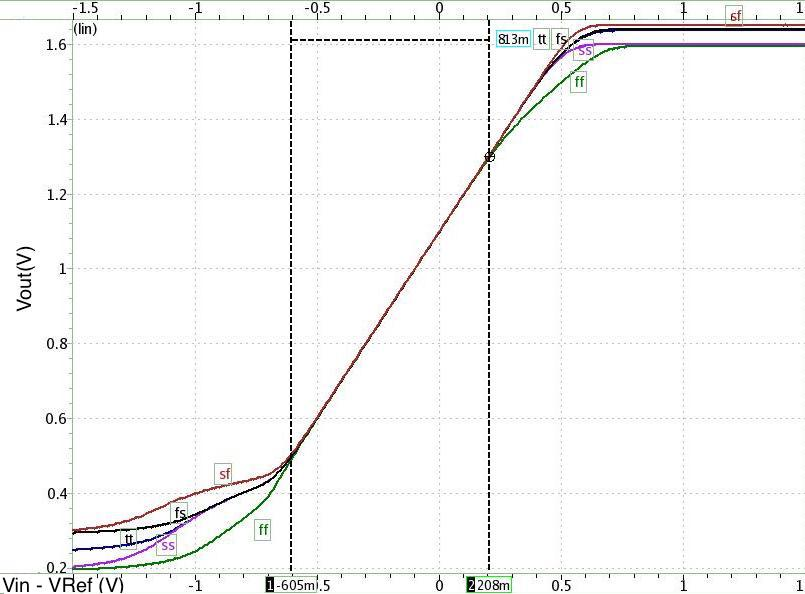
\includegraphics[width=1\textwidth] {images/chapter5/postSim/subtractor_5_xx.PNG}
        \raggedleft
        (a)
    \end{minipage}
    \vfill
    \begin{minipage}[t]{1\textwidth}
        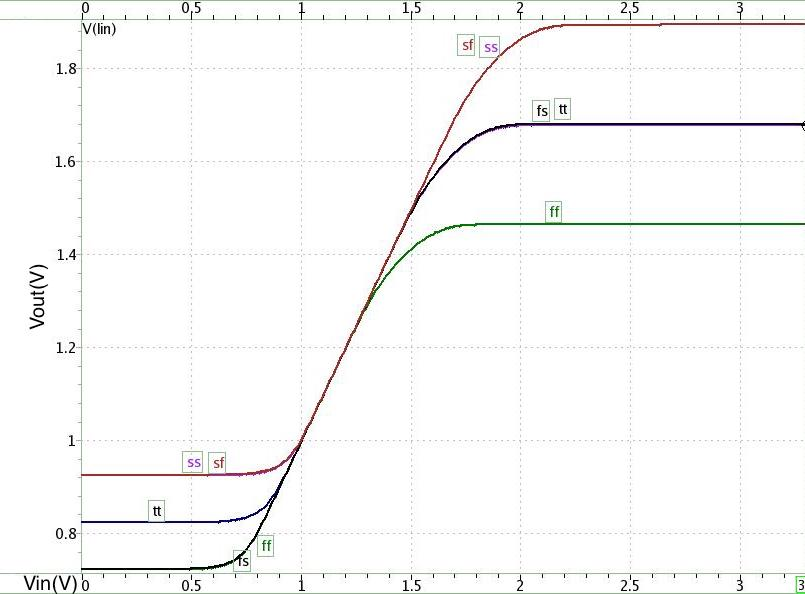
\includegraphics[width=1\textwidth] {images/chapter5/postSim/subtractor_5_zz.PNG}
        \raggedleft
        (b)
    \end{minipage}
    \caption{DC response of the output of our analog subtractor. (a)The x-axis is the difference between positive input and negative input ($V_x - V_{Ref}$). (b) The x-axis is the voltage of $v_z$ }
    \label{fig:sim:subtractor}
\end{figure}


\begin{table}[!htb]
    {\fontfamily{}\fontsize{10}{14}\selectfont
    \centering
    \begin{tabular}{l|c|c}
        & $V_x$ & $V_z$\\
        \hline
        Input Dynamic Range & $V_{Ref} - 0.57$-$V_{Ref} + 0.2$ & $1$-$1.38$ \\
        \hline
        Bandwidth & 675k Hz& - \\
        \hline
        SNR (@10Hz) & 8.3e10 & 8.4e10 \\
    \end{tabular}
    \caption{The summary table of the analog subtracter circuit.}
    \label{tb:Subtractor}
    }
\end{table}

\subsection{Non-inverting Resistor-based Amplifier}

\begin{figure}[!htbp]
    \centering
        \includegraphics[width=0.5\textwidth] {images/chapter5/ResAmp.png}
    \caption{The non-inverting resistor-based amplifier circuit}
    \label{fig:ResAmp}
\end{figure}

Fig.\ref{fig:ResAmp} is the last block of the second stage circuit.
It is a non-inverting resistor-based Amplifier.
We adopt this simple structure to amplify the output signal of the subtractor.
When the subtractor sends a small signal $\Delta v$ into Vin, the output voltage ($v_{out}$) is:
\begin{align}
    v_{out} &= (\Delta v - v_f) \times A_{Op2} \\
    v_f &= v_{out} \frac{R_i}{R_o + R_i} \\
    \frac{v_{out}}{\Delta v} &= \frac{A_{Op2}}{1 + A_{Op2}\frac{R_i}{R_i + R_o}} \\
    &\approx \frac{R_i + R_o}{R_i} \quad \text{For} \quad \frac{R_iA_{Op2}}{R_i + R_o} > 10 \label{eq:ResAmp}
\end{align}
The $R_i$ can be  $110k\Omega$ or $9.2k\Omega$ ($10k\Omega||110k\Omega$).
(When two switches is off, the circuit act like a unit-gain buffer.)
Eq.(\ref{eq:ResAmp}) suggests that the $A_{Op2}$ should be larger than 1000 (60dB).
Thus, the Op2 in Fig.\ref{fig:ResAmp} adopts the structure of two-stage differential pair (same with the operational amplifier in TIA block) due to its high gain and wide output dynamic range (rail-to-rail).

One thing to note is that the derivation above views the $V_z$ as the virtual ground.
The $V_z$ equals to the offset voltage of $V_{in}$.
And it is the output offset voltage of the amplifier as well.
In fact, this results in the input dynamic range of $\frac{\pm V_z}{Amplification Rate}$. (As long as the Op2 is a rail-to-rail operational amplifier).
This emphasizes the importance of the subtractor block.
If we directly connect the input of the amplifier to the fist stage output, the input dynamic range will be $\frac{\pm V_{Ref}}{Amplification Rate}$.
The $V_{Ref}$ is around $\pm 1V$ and is lower than $V_z$.

Fig.\ref{fig:sim:ResAmp} presents the five corners post-simulation results of the amplifier.
We swept the input and measured the output under three amplification rate.
And Table.\ref{tb:sim:ResAmp} is the summary table.

\begin{figure}[!htbp]
    \begin{minipage}[t]{1\textwidth}
        \centering
        \includegraphics[width=0.8\textwidth] {images/chapter5/postSim/ResAmp_1.PNG}
        \raggedleft
        (a)
    \end{minipage}
    \vfill
    \begin{minipage}[t]{1\textwidth}
        \centering
        \includegraphics[width=0.8\textwidth] {images/chapter5/postSim/ResAmp_10.PNG}
        \raggedleft
        (b)
    \end{minipage}
    \vfill
    \begin{minipage}[t]{1\textwidth}
        \centering
        \includegraphics[width=0.8\textwidth] {images/chapter5/postSim/ResAmp_100.PNG}
        \raggedleft
        (c)
    \end{minipage}
    \caption{Five corners output DC response (vout) and derivative ($dvout/dvin$) when being operated under the amplification rate of (a)1, (b)10, (c)100.}
    \label{fig:sim:ResAmp}
\end{figure}


\begin{table}[!htb]
    {\fontfamily{}\fontsize{10}{14}\selectfont
    \centering
    \begin{tabular}{l|c|c|c}
        Amplification Rate & 100 & 10 & 1\\
        \hline
        Error & < 7\% & < 0.7\% & < 0.02\% \\
        \hline
        Bandwidth & 210k Hz & 190k Hz & 2M Hz\\
        \hline
        Input Dynamic Range & from $-9mV$ to $17mV$ & from $-0.11V$ to $0.14V$ & from $-0.5$ to $0.3V$\\
        \hline
        Output Dynamic Range & \multicolumn{3}{c}{$0.1V$ - $3V$}\\
    \end{tabular}
    \caption{The summary table of simulation results.}
    \label{tb:sim:ResAmp}
    }
\end{table}

\FloatBarrier

\section{post-simulation Result of the Transient Measurement mode circuit}
As mentioned in section.\ref{sec:TrM}, there are two usage of the Transient Measurement mode circuit (Fig.\ref{fig:ACmode}).
There simulation results are presented sperately below.

\subsection{Input from Gate}

\begin{figure}[!htbp]
    \centering
        \includegraphics[width=0.7\textwidth] {images/chapter5/NWROC_block_vg.png}
    \caption{The block diagram of the Transient Measurement circuit. We simulate it by sending ac signal through the voltage source Vg.}
    \label{fig:Nblockvg}
\end{figure}

The first usage is to detect the output response of input voltage signal at gate.
The voltage signal is caused by the the biomolecule concentration.
This measurement are usually preceded by the DC-Sweep mode, which initialize the $I_D$ with the value of Ibias and set $g_m$ to a corresponding value.
Therefore, we replaced the transistor elements and Vg by a current signal Iin as in Fig.\ref{fig:Nblockvg}.
And we apply an ac signal from Iin to perform the ac analysis.

\begin{figure}[!htb]
    \centering
        \includegraphics[width=1\textwidth] {../images/chapter5/postSim/totalGain.PNG}
    \caption{The gain of $\frac{V_{out}}{I_{in}}$ when the amplification rate of the second stage is 100.}
    \label{fig:sim:vgGain}
\end{figure}

\begin{figure}[!htb]
    \centering
        \includegraphics[width=1\textwidth] {../images/chapter5/postSim/noise.png}
    \caption{The input referred noise when the amplification rate of the second stage is 100.}
    \label{fig:sim:vgnoise}
\end{figure}

Fig.\ref{fig:sim:vgGain} presents the maximum gain that the circuit in five corners provides.
And Fig.\ref{fig:sim:vgnoise} is input referred noise analysis.
The design spec requires the gain to be greater than $5E6$ and the voltage noise referred to the gate of nanowire to be smaller than $2mV$.
The summary table (Table.\ref{tb:sim:vg}) computed the noise result by considering the $g_m$ as $200n$, which is the minimum $g_m$ that may exist in our measurement.

\begin{table}[!htbp]
    {\fontfamily{}\fontsize{10}{14}\selectfont
    \centering
    \begin{tabular}{l|c|c}
        & Design Spec (Table.\ref{tb:ACSpec}) & Simulation Result \\
        \hline
        Amplification Rate (max)& $5E6$ & $1.03E7$\\
        \hline
        Input Referred Noise & $< 2m V$ & $ = \frac{\sqrt{5.8E-20}}{200n}$ = $1.2m V$ @1Hz
    \end{tabular}
    \caption{The summary table. The simulation results are compared with the design spec.}
    \label{tb:sim:vg}
    }
\end{table}

\subsection{Input from Source}
\begin{figure}[!htbp]
    \centering
        \includegraphics[width=0.7\textwidth] {images/chapter5/NWROC_block_vs.png}
    \caption{The block diagram of the Transient Measurement circuit. We simulate it by sending ac signal to the source of the nanowire.}
    \label{fig:Nblockvs}
\end{figure}

The second usage of the Transient Measurement mode circuit is to apply a sinusoidal voltage signal at the source of nanowire.
The Vg and Ibias are fixed at constant during the measurement.
The output voltage is measured and used for computing the $g_m$ of the element.
\begin{equation}
    g_m = frac{V_{out}}{v_s \times R_{TIA} \times A_{second}}
\end{equation}
The $v_s$ is the amplitude of the input sinusoidal signal.
And the $A_{second}$ is the amplification rate of the second stage circuit.

One thing to be noted is the offset voltage of the output.
The biomolecule concentration difference changes the $I_D$ of nanowire.
This $I_D$ difference not only results in the changes of $g_m$ but also alter the offset current flowing through the $R_{TIA}$.
This current is also amplified and may cause the output saturation.
The solution is to utilize Ibias to cancel the offset current.

We can find the limit of the offset current.
Since the output dynamic range of the resistor-based amplifier is from $0V$ to $3V$, the limit is $\pm \frac{1.5V}{A_{amp} \times R_{TIA}}$ where the $A_{amp}$ is 1, 10 or 100.

Two simulation results presented below are the transient response of the output voltage when the $A_{amp}$ is 10 (Fig.\ref{fig:sim:sine10})and 100(Fig.\ref{fig:sim:sine100}).
The $g_m$ of the transistor is swept in the same time.
The input sinusoidal signal has frequency of $1k$Hz and amplitude of $20mV$.
Their corresponding ac sweep is presented in Fig.\ref{fig:sim:sine10_ac} and Fig.\ref{fig:sim:sine100_ac}.
This results show that the circuit bandwidth is about $10k$.

\begin{figure}[!htbp]
    \centering
        \includegraphics[width=1\textwidth] {images/chapter5/postSim/sine_gm_x10_1u_10u_tran.PNG}
    \caption{The transient analysis. The amplification rate of $A_{amp}$ is 10. The $g_m$ is swept from $1\mu$ to $10\mu$.}
    \label{fig:sim:sine10}
\end{figure}
\begin{figure}[!htbp]
    \centering
        \includegraphics[width=1\textwidth] {images/chapter5/postSim/sine_gm_x10_1u_10u_ac.PNG}
    \caption{The ac analysis of the transient simulation result in Fig.\ref{fig:sim:sine10}.}
    \label{fig:sim:sine10_ac}
\end{figure}

\begin{figure}[!htbp]
    \centering
        \includegraphics[width=1\textwidth] {images/chapter5/postSim/sine_gm_x100_1u_6u_tran.PNG}
    \caption{The transient analysis. The amplification rate of $A_{amp}$ is 100. The $g_m$ is swept from $1\mu$ to $6\mu$. There are two curves have the output saturation problem. One solve it by increasing the current provided by Ibias.}
    \label{fig:sim:sine100}
\end{figure}
\begin{figure}[!htbp]
    \centering
        \includegraphics[width=1\textwidth] {images/chapter5/postSim/sine_gm_x100_1u_6u_ac.PNG}
    \caption{The ac analysis of the transient simulation result in Fig.\ref{fig:sim:sine100}.}
    \label{fig:sim:sine100_ac}
\end{figure}





%